%% CS2640 Modern Storage Systems --- Final Project Report

\documentclass[letterpaper,twocolumn,10pt]{article}
\usepackage{usenix-2020-09}
\usepackage{graphicx}
\usepackage{booktabs}
\usepackage{amsmath}
\usepackage{listings}
\usepackage{multirow}
\usepackage{tabularx}
\usepackage[shortlabels]{enumitem}
\usepackage[normalem]{ulem}
\usepackage{float}
\usepackage{xcolor}
\usepackage{caption}

\graphicspath{{figures/}}

\lstset{
  basicstyle=\ttfamily\scriptsize,
  breaklines=true,
  frame=single,
  backgroundcolor=\color{gray!8},
  rulecolor=\color{gray!40},
  xleftmargin=4pt, xrightmargin=4pt,
}

\newcommand{\sysname}{AdaptiveCache}
\newcommand{\para}[1]{\smallskip\noindent\textbf{#1.}\ }
\newcommand{\etal}{\textit{et al.}}

\begin{document}
\date{}

\title{\Large \bf AdaptiveCache: A Lifetime-Cost Study of Context Management
       for LLM Agents under Prefix-Cache-Aware Pricing}

\author{
  {\rm Vlad Cainamisir}\\
  Harvard John A. Paulson School of Engineering and Applied Sciences\\
  {\small CS2640: Modern Storage Systems\quad---\quad Final Report, May 2026}
}

\maketitle

\begin{abstract}
LLM agents accumulate tens of thousands of tokens across long
tool-use trajectories. Modern serving systems exploit prefix caching,
billing already-computed tokens at roughly $1/10$ the cost of
uncached input. Compaction policies that drop ``stale'' context
therefore look like obvious wins. We test some training-free
versions of this hypothesis empirically. Across \textbf{eight
heuristic compaction policies, $\sim$30 distinct task instances}
(SWE-bench Lite live, $\tau$-bench retail with chain extension), and
\textbf{two model classes} (Qwen3-30B-A3B local, Anthropic Haiku 4.5
API), \textbf{no policy we tested Pareto-dominates \texttt{none}} (no
compaction). The cause is a \emph{cliff tax}: every compaction event
mutates the prompt prefix, invalidates all downstream chain-hashed
cache blocks, and re-bills the suffix at the uncached rate on the
next call. We derive that compaction needs $\sim$45 remaining steps
to break even per compaction event; most agent trajectories from our chosen benchmarks have far
fewer. We then present the constructive direction the negative result
motivates: a system that captures observation KV to CPU on
compaction, restores it on recall, and rotates the suffix's
already-cached K vectors in place by $\Delta$ tokens via the rotary
composition identity $R(p+\Delta) = R(\Delta) \circ R(p)$, combined
with an append-only auxiliary chain-hash registration that makes the
cached blocks reachable under the recall-prompt's chain hash. The
mechanism is end-to-end operational on an H100 with the rotation
correctness verified to bf16 cosine similarity $>$0.999 across
layers.
\end{abstract}

\section{Introduction}
\label{sec:intro}

Long-running LLM agents---ReAct~\cite{yao2023react}, OpenHands, Claude
Code---accumulate context across hundreds of tool calls. Every tool
observation is appended to the conversation; the entire conversation
is re-sent to the inference server every step. Without compaction the
prompt grows unboundedly, eventually exceeding model context length
and inflating per-step cost.

The prevailing assumption is that compaction is good for cost. The
argument is intuitive: tool observations from many steps ago are
usually no longer needed; dropping them shortens the prompt. Many
systems implement this---summarization at budget
(OpenHands~\cite{openhands2025}), attention-based KV
eviction~\cite{zhang2023h2o,xiao2024streamingllm,li2024snapkv},
RL-distilled state replacement~\cite{zhou2025mem1,yu2025memagent},
context folding~\cite{sun2025contextfolding}.

\textbf{The argument is incomplete.} On modern serving systems, input
tokens are billed at \emph{two rates}: a cheap rate for tokens whose
KV state is already cached server-side, and a $\sim$10$\times$ more
expensive rate for tokens whose KV state must be computed afresh.
Cache reuse is keyed on byte-identical prefixes. Any compaction
event modifies the prefix, invalidates downstream cache, and forces
recomputation at the expensive rate.

This is the question the project asks: \textbf{when the cost of
\emph{changing} the prefix is $\sim$10$\times$ the cost of \emph{not
changing} it, can a heuristic compaction policy still Pareto-dominate
not compacting at all?}

\noindent We answer across multiple benchmarks, models, and policies.
The answer, for our chosen benchmarks and models, is \textbf{no}. Given our limited budget, we were not able to run on long context benchmarks. On tasks under 100k tokens, compaction is a net negative.

\para{Contributions} (1) A lifetime-cost evaluation framework that
attributes per-step costs to compaction events across five provider
price columns. (2) An empirical demonstration that no training-free
heuristic compaction policy in our 8-policy survey beats
\texttt{none} at the scale tested. (3) A back-of-envelope
derivation of the cliff tax that explains \emph{why}. (4) An
inference-engine overlay that combines KV capture/restore with
in-place rotary K-vector rotation and append-only auxiliary
chain-hash registration---making the cached suffix reachable and
\emph{correct} under the recall-prompt's chain hash, without
re-prefilling. (5) An honest accounting of what we have shown
(mechanism) and what we have not (Pareto win on a real workload).

\para{Terminology} A \emph{tool observation} (or just
\emph{observation}) is the text returned by an agent's tool call
(e.g.\ the contents of a \texttt{read\_file}), appended to the
conversation. \emph{Compaction} is any operation that shortens
the agent's prompt by removing, summarizing, or substituting an
older observation. The \emph{prefix} is the front of the request
prompt and the \emph{suffix} is its tail; cache reuse depends on
prefix bytes being identical across requests. The \emph{KV cache}
is the set of per-token Key/Value attention activations the
inference server keeps to avoid re-running the model forward on
already-seen tokens. \emph{Recall} is the inverse of compaction:
re-introducing a previously compacted observation back into the
prompt. A policy \emph{Pareto-dominates} \texttt{none} on a
workload if it resolves at least as many tasks at strictly lower
cost.

% =====================================================================
\section{Background}
\label{sec:background}

\subsection{Prefix caching and the storage analogy}

Modern inference servers (vLLM~\cite{kwon2023pagedattention},
SGLang~\cite{zheng2024sglang}, Anthropic, OpenAI) implement prefix
caching: blocks of KV state are keyed by a chained content hash
$H_i = \mathrm{hash}(H_{i-1}, \mathrm{tokens}_i)$. Two consecutive
requests sharing a byte-identical prefix reuse the cached blocks; the
first divergent block triggers a cache miss and forces re-prefill of
everything after.

Concretely, in a vLLM-style engine: the \emph{scheduler} assigns
each request to a pool of fixed-size \emph{KV blocks} on the GPU;
a per-request \emph{block table} maps logical token positions to
the physical block IDs that hold their K and V activations; and
a global \emph{prefix-cache hash table} maps chain hashes $H_i$
to the physical blocks that contain their content. When a
request arrives, the scheduler walks the request's chain hashes
against the prefix-cache hash table and reuses any matching
blocks; only the first uncached position onward is prefilled.

This is the storage-systems pattern the course studies: a
content-addressable cache with locality-driven reuse, where the
\emph{layout} of items (their byte position in the prompt)
determines hit rate. \emph{What} you keep matters; so does
\emph{where} it sits.

\subsection{The original \sysname{} thesis and prior measurements}

Existing eviction
methods~\cite{zhang2023h2o,xiao2024streamingllm,li2024snapkv,
liu2023scissorhands,cai2024pyramidkv} optimize \emph{what to keep};
\sysname{} would also optimize \emph{where to put it}, pinning
stable high-value items at fixed prefix positions and demoting
volatile items to the suffix.

\para{Trace-driven measurements informing the design} Before
running any policy comparison we measured four properties of
real agent trajectories on the Hermes Agent Reasoning Traces
corpus. (i)~Three candidate importance proxies---how often a
span is referenced by later tokens, semantic similarity to the
goal, and attention weight from later positions---are pairwise
near-zero correlated, so no single proxy captures ``which token
matters.'' (ii)~Across Qwen3 0.6B--8B, the first 10\% of token
positions carry 500--1500$\times$ more aggregate attention mass
than the rest (\emph{position primacy}), motivating a stable
prefix zone. (iii)~Tool observations are 77\% of agent-loop
tokens, and large observations receive proportional
attention---size alone is the wrong eviction signal. (iv)~On
production Anthropic Haiku trajectories, each compaction event
costs \$0.10--\$0.15 of new uncached input on the next call and
needs $\sim$5+ steps to amortize. We work the underlying
arithmetic out in \S\ref{sec:cliff_tax}.


\subsection{Related work}

Table~\ref{tab:related} compares \sysname{} to existing systems on
three properties relevant to our cost model.

\begin{table}[h]
\centering\small
\setlength{\tabcolsep}{4pt}
\begin{tabular}{lccc}
\toprule
\textbf{System} & \textbf{Train.} & \textbf{Layout} & \textbf{Cache} \\
                & \textbf{free?}  & \textbf{aware?} & \textbf{aware?} \\
\midrule
FIFO / LRU                              & Yes & No  & No \\
H2O, SnapKV, ScissorHands, PyramidKV    & Yes & No  & No \\
StreamingLLM~\cite{xiao2024streamingllm}                  & Yes & Partial & Partial \\
LLMLingua~\cite{jiang2023llmlingua,jiang2024longllmlingua}  & Optional & No & No \\
ReSuM~\cite{wu2025resum}                                  & Yes & No  & No \\
SUPO~\cite{lu2025supo}                                    & RL  & No  & No \\
MEM1~\cite{zhou2025mem1}                                  & RL  & No  & No \\
MemAgent~\cite{yu2025memagent}                            & RL  & No  & No \\
Context Folding~\cite{sun2025contextfolding}              & RL  & No  & Partial \\
MEMENTO~\cite{kontonis2026memento}                        & SFT & No  & Partial \\
Claude Code~\cite{claudecode2025}                         & Yes & Partial & \textbf{Yes} \\
\midrule
\textbf{\sysname{} (proposed)}                            & \textbf{Yes} & \textbf{Yes} & \textbf{Yes} \\
\bottomrule
\end{tabular}
\caption{\sysname{} relative to existing context-management systems.
Claude Code is the only prior system with all three properties.}
\label{tab:related}
\end{table}

% =====================================================================
\section{Lifetime-cost framework}
\label{sec:framework}

We define lifetime cost per task as the sum of per-step
input/output costs across the trajectory plus any summarizer-LLM
costs incurred by compaction:
\[
\mathrm{lifetime\_\$}(\tau) = \sum_t \big(
  u_t p_u + c_t p_c + o_t p_o + w_t p_w
\big) + \sum_e s_e
\]
$u_t$, $c_t$, $o_t$, $w_t$ are uncached / cached / output /
cache-write tokens at step $t$; prices come from a per-provider
price table; $s_e$ is the cost of a compaction-time summarizer
call. This metric captures the cost of \emph{changing} the
prefix, which dominates for any policy that fires.

\subsection{Evaluation methodology}
\label{sec:evaluation_method}

Each SWE-bench Lite task ships with a \texttt{base\_commit} (the
pre-fix state of the repository), a \texttt{test\_patch} (the
regression tests added alongside the maintainers' fix), and two
named test lists: \texttt{FAIL\_TO\_PASS} (tests that should pass
after the bug fix) and \texttt{PASS\_TO\_PASS} (tests that should
remain passing). We resolve a trajectory against this same gold
set. For each completed trajectory we (1)~replay its
\texttt{edit\_file} calls onto a fresh git checkout at
\texttt{base\_commit}, (2)~apply the \texttt{test\_patch} on top,
(3)~provision a per-instance Python~3.9 venv (\texttt{uv} as the
package manager), (4)~run \texttt{pytest} on the
\texttt{FAIL\_TO\_PASS} list, and (5)~declare the trajectory
resolved iff every \texttt{FAIL\_TO\_PASS} test passes and no
\texttt{PASS\_TO\_PASS} test regresses.

\subsection{How this differs from the standard harness}
\label{sec:disclosures}

Three differences are worth flagging upfront.

\para{No docker} The official harness containerizes each instance.
We do not, because our evaluation runs inside Modal and Modal does
not support docker-in-docker. We instead use \texttt{uv}-managed
Python~3.9 venvs per instance (many SWE-bench Lite
\texttt{base\_commit}s do not build under Python~3.12). All tasks
in our task list (psf/requests, pallets/flask, pylint, pytest)
provision and execute under this setup.

\para{Test-patch collisions are unvalidatable} If the agent's
edits touch the same lines \texttt{test\_patch} adds, the patch
fails to apply and the trajectory cannot be validated. We report
both the full-set count and the validatable-subset count
(e.g., 5/10 and 5/7) and use the latter for cross-policy
comparison.

\para{Single seed at $N{=}10$} Our main run is single-seed. At
this scale a single task's outcome moves the resolve count by ten
percentage points; \$/resolved divides by an integer denominator
and is correspondingly noisy. We use it only alongside total \$
and the validatable-subset resolve count, and do not draw causal
claims from \$/resolved differences that hinge on $\le$1 task.

% =====================================================================
\section{Compaction policies under test}
\label{sec:policies}

\begin{figure*}[t]
  \centering
  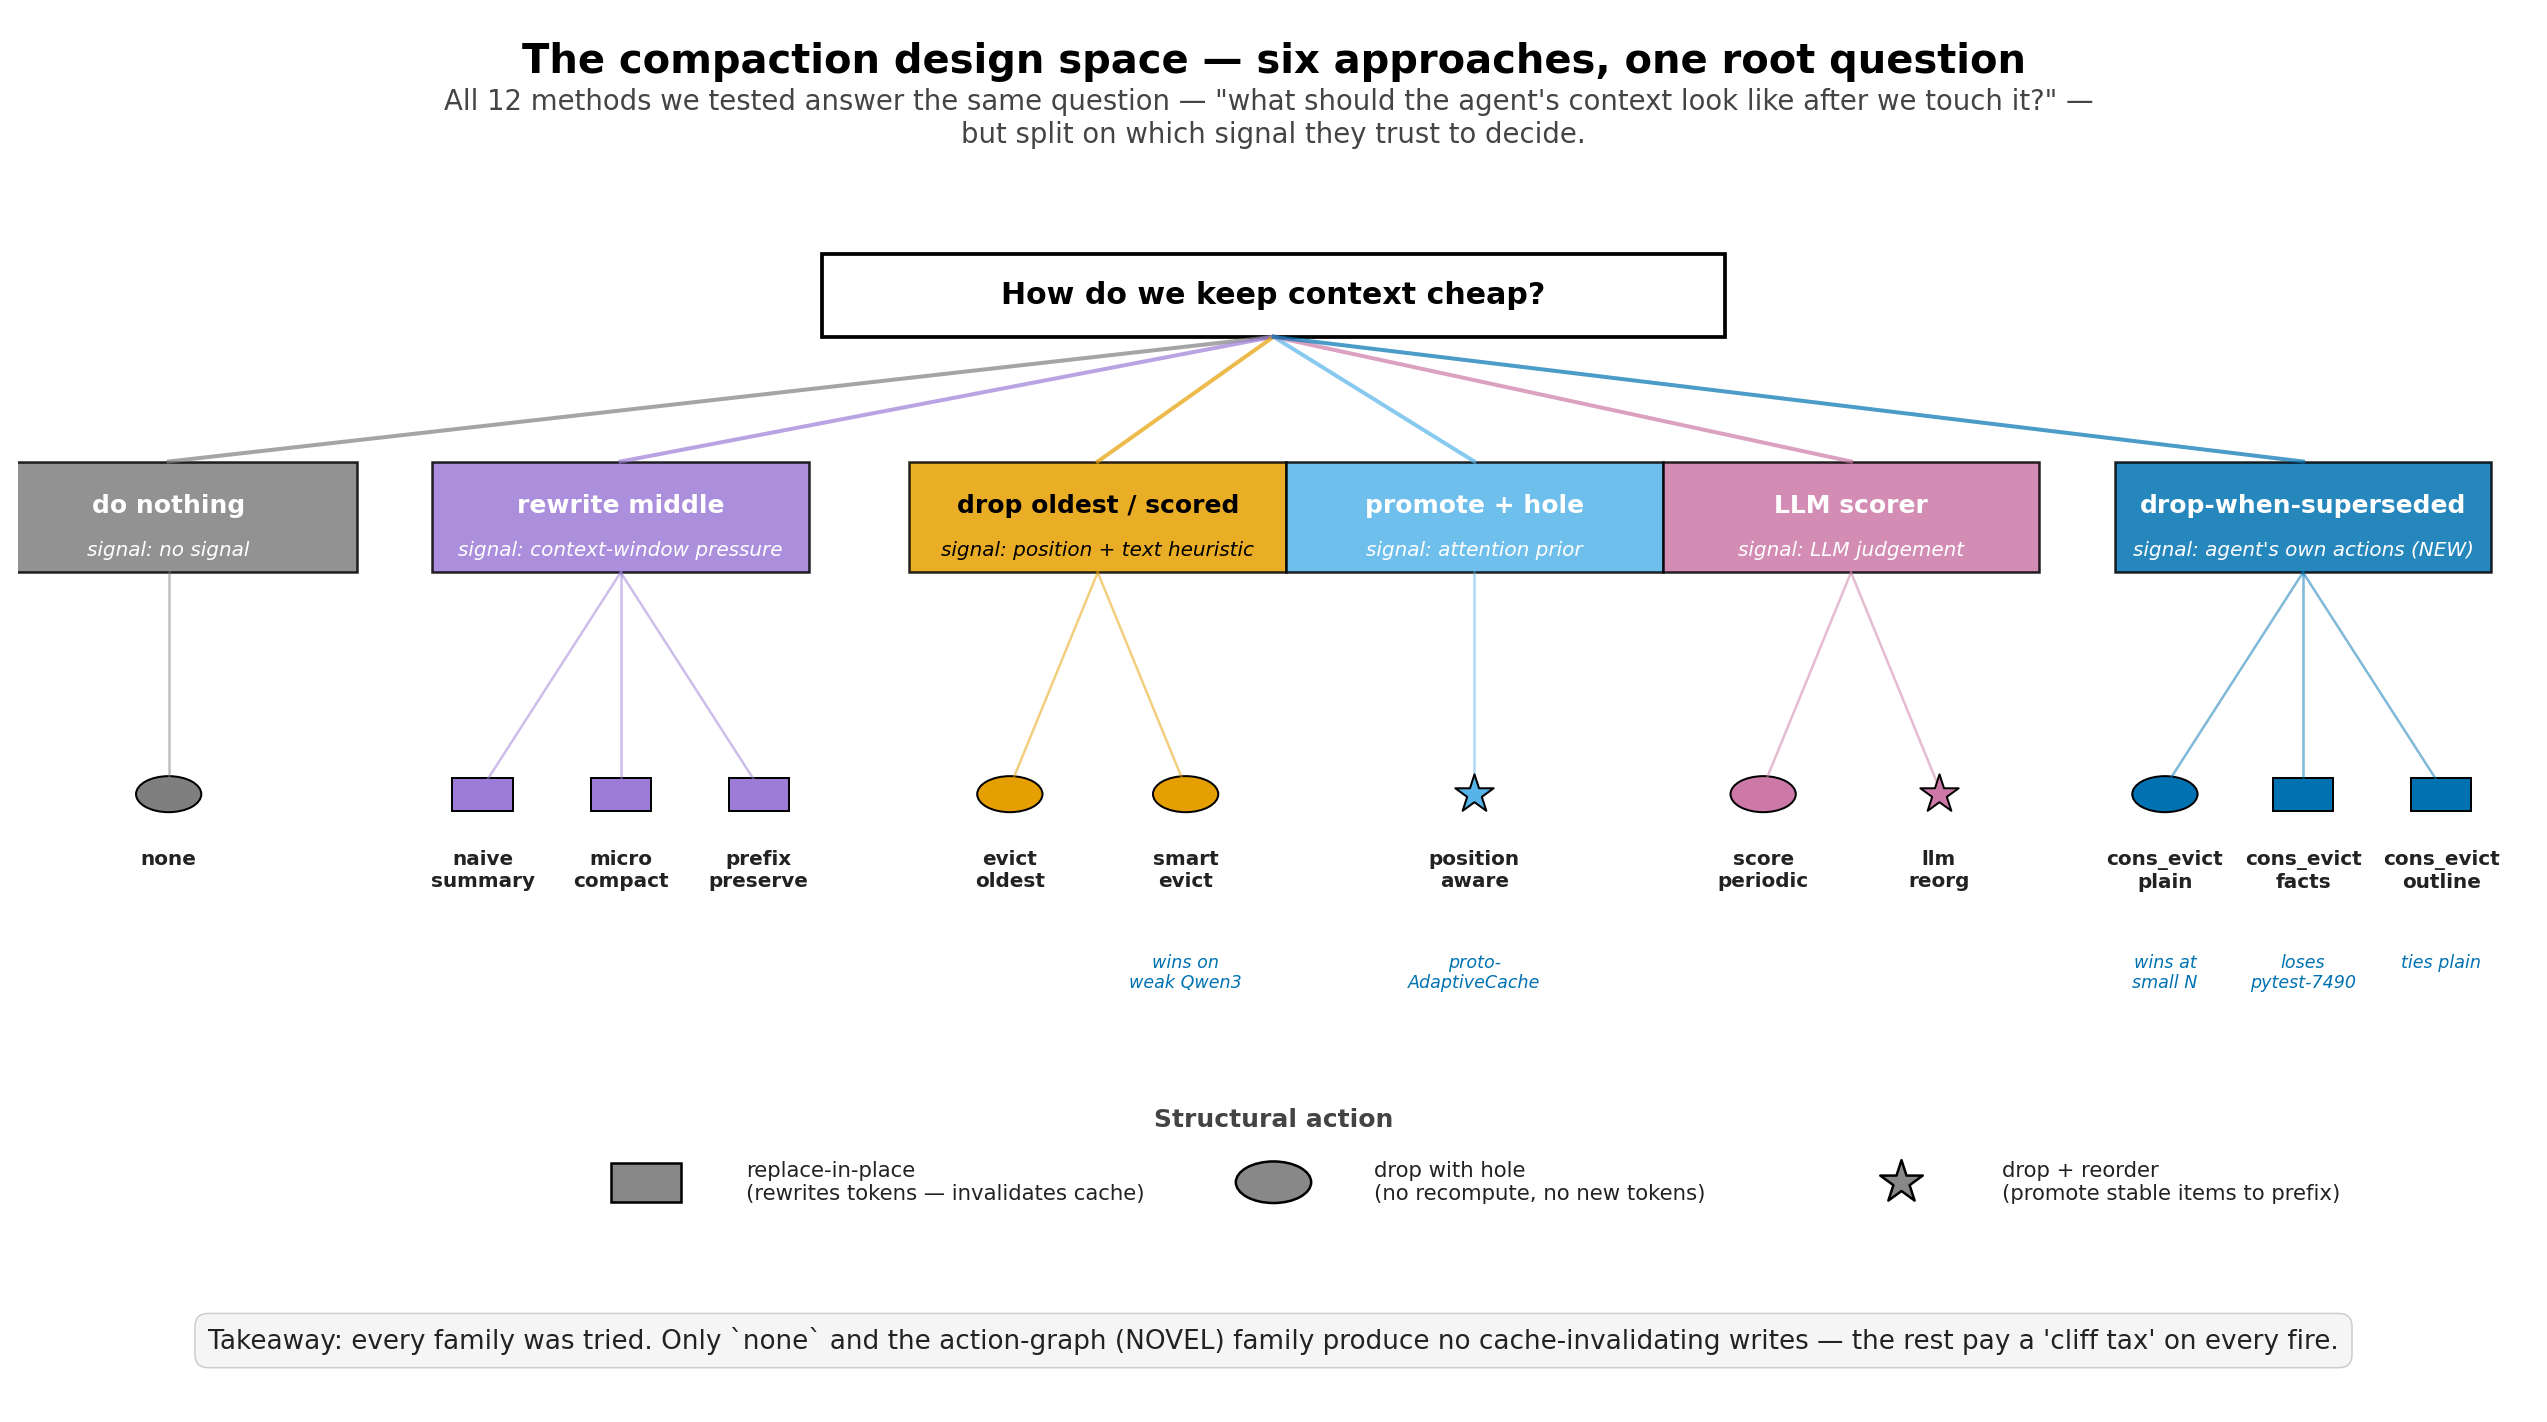
\includegraphics[width=0.92\textwidth]{fig9_method_family_tree.png}
  \caption{The eight training-free compaction policies tested. The
  rightmost branch (\texttt{consumption\_evict} family) is novel:
  observations are tagged consumed by subsequent agent actions (e.g., a
  read followed by an edit on the same path consumes the read).
  Three placeholder-content variants are evaluated under the same
  eviction signal (\S\ref{sec:placeholder}).}
  \label{fig:methods}
\end{figure*}

We implemented eight training-free compaction policies covering
the natural design space (Figure~\ref{fig:methods}). Each policy
fires when the rendered prompt exceeds a soft token budget; what
differs is \emph{which} observations are dropped and \emph{what,
if anything,} replaces them. Table~\ref{tab:policy_summary} gives
the one-line mechanism for each, alongside how the policy fared
in our empirical run.

\begin{table*}[t]
\centering\small
\setlength{\tabcolsep}{6pt}
\begin{tabular}{p{0.18\textwidth} p{0.42\textwidth} p{0.32\textwidth}}
\toprule
\textbf{Policy} & \textbf{Mechanism} & \textbf{Observed in our runs} \\
\midrule
\texttt{none} &
Identity. No compaction. &
Baseline; on the Pareto frontier. \\

\texttt{evict\_oldest} (FIFO) &
Drop the oldest tool observation when the prompt exceeds the soft budget. &
Matches \texttt{none} resolve only with 2--3$\times$ more steps; cost dominated by the cliff on each fire. \\

\texttt{naive\_summary} &
Concatenate all observations between the system prompt and the recent $M$ turns; replace them with one summary message produced by a small LLM. &
Summariser cost stacked on the cliff; consistently dominated. \\

\texttt{microcompact} &
Rewrite each oversized observation in place to a 1--2 line summary; conversation structure preserved. &
Same cost shape as \texttt{naive\_summary}; never on the frontier. \\

\texttt{prefix\_preserving} &
Freeze the first $K$ turns as a stable prefix; replace the middle with one summary; keep the most recent $M$ turns verbatim. &
+200\% cost vs \texttt{none} on the four heavy tasks (Table~\ref{tab:cost_decomp}); 19 summariser calls + 19 cliffs. \\

\texttt{position\_aware} &
Drop oldest, but leave a fixed \texttt{[evicted]} placeholder in the message slot rather than removing it. &
Same Pareto profile as FIFO; the placeholder does not save the cliff. \\

\texttt{smart\_evict} (type-prior) &
Rank eviction candidates by combining a per-tool-type prior (file reads $>$ search results) with a textual-overlap reference count from later turns; drop the lowest-ranked. &
+67\% cost vs \texttt{none} at equal resolves on the four heavy tasks. \\

\texttt{llm\_reorganizer} &
A small LLM scores each tool observation 1--10 for likely future relevance; drop the $K$ lowest-scored. &
+39\% cost vs \texttt{none} at equal resolves; the auxiliary LLM is the cheapest summariser-call profile we tried but still loses. \\

\texttt{consumption\_evict} \newline (action-graph supersession) &
Tag tool observations as \emph{consumed} via tool-call semantics; drop only confirmed-stale observations. Five rules: \texttt{read\_file}$\to$\texttt{edit\_file} on same path; \texttt{search}$\to$\texttt{read\_file} on same path; consecutive \texttt{run\_tests}; \texttt{edit\_file} consuming prior reads of same file; \texttt{submit} consuming everything. &
+120\% cost vs \texttt{none} at equal resolves on the headline run (Table~\ref{tab:main_result}); the cost-cheapest compaction policy in our survey but still dominated. \\
\bottomrule
\end{tabular}
\caption{The eight training-free compaction policies under test.
Each fires when the prompt exceeds a soft budget; the
\textbf{Mechanism} column states what each policy does on a fire,
the \textbf{Observed} column states how it fared empirically.
None are on the Pareto frontier alongside \texttt{none}.}
\label{tab:policy_summary}
\end{table*}

To our knowledge no prior compaction system uses tool-graph
supersession; the \texttt{consumption\_evict} family is novel
and works mechanistically (it correctly tags consumed
observations across all 60+ trajectories we inspected) but the
cliff tax dominates its byte savings (\S\ref{sec:cliff_tax}).

\subsection{Benchmarks}

We tested on (a) \textbf{SWE-bench Lite}, a coding-agent
benchmark where the agent must produce a patch that passes the
maintainers' regression tests; we use a no-docker reimplementation
of the harness in which the agent operates against a cloned
repository through six tools (\texttt{list\_files},
\texttt{read\_file}, \texttt{search}, \texttt{edit\_file},
\texttt{run\_tests}, \texttt{submit}). And (b) \textbf{$\tau$-bench}
retail, a customer-service multi-turn dialogue benchmark; we extend
it with a multi-customer chain harness that bundles $N$ consecutive
customer tasks into one continuous agent session
(\texttt{chain\_size}=$N$).

An initial run on $\tau$-bench's airline domain showed it to be
the wrong benchmark for this study: single-customer tasks fit
naturally in 16K, prefix-cache hit rate is already $\sim$95\%,
and observations cap at 950 tokens. \emph{There is nothing to
compact}, and policies that trigger end up 6$\times$ more
expensive than \texttt{none}. We moved on.

% =====================================================================
\section{Empirical results}
\label{sec:results}

\subsection{Main result: no policy beats \texttt{none}}

\begin{table*}[t]
\centering\small
\setlength{\tabcolsep}{6pt}
\begin{tabular}{lcccccc}
\toprule
\textbf{Policy} & \textbf{Real-resolved} & \textbf{Validatable} & \textbf{Total \$} & \textbf{\$/resolved} & \textbf{Compactions} & \textbf{Mean steps} \\
\midrule
\texttt{none}                                   & 5/10 & 5/7 (71\%) & \textbf{3.47} & \textbf{0.69} &  0 & 25.5 \\
\texttt{consumption\_evict} (plain)             & 5/10 & 5/7 (71\%) & 7.63 & 1.53 & 31 & 30.6 \\
\texttt{consumption\_evict\_facts}              & 4/10 & 4/8 (50\%) & 6.15 & 1.54 & 26 & 32.5 \\
\texttt{consumption\_evict\_outline}            & 5/10 & 5/7 (71\%) & 8.16 & 1.63 & 32 & 32.4 \\
\bottomrule
\end{tabular}
\caption{Main result. Haiku 4.5, $N{=}10$ SWE-bench Lite, single
seed, \texttt{FAIL\_TO\_PASS} validation. The cheapest compaction
variant costs 2.2$\times$ more than \texttt{none} for the same
resolve count. \textbf{No policy in our survey
Pareto-dominates \texttt{none} at this scale.}}
\label{tab:main_result}
\end{table*}

Table~\ref{tab:main_result} and Figure~\ref{fig:pareto} report the
main negative result. The cheapest compaction variant costs
2.2$\times$ more than \texttt{none} for the same resolve count.
Cost decomposition (Figure~\ref{fig:cost_decomp}) shows the cost
killer is \texttt{input\_uncached}; Table~\ref{tab:cost_decomp}
gives the same view restricted to \emph{four heavy SWE-bench Lite
tasks} (a subset of the slate above), the regime where
\texttt{prefix\_preserving} actually fires often enough for the
per-line-item dollars to be meaningful.

\begin{figure}[h]
  \centering
  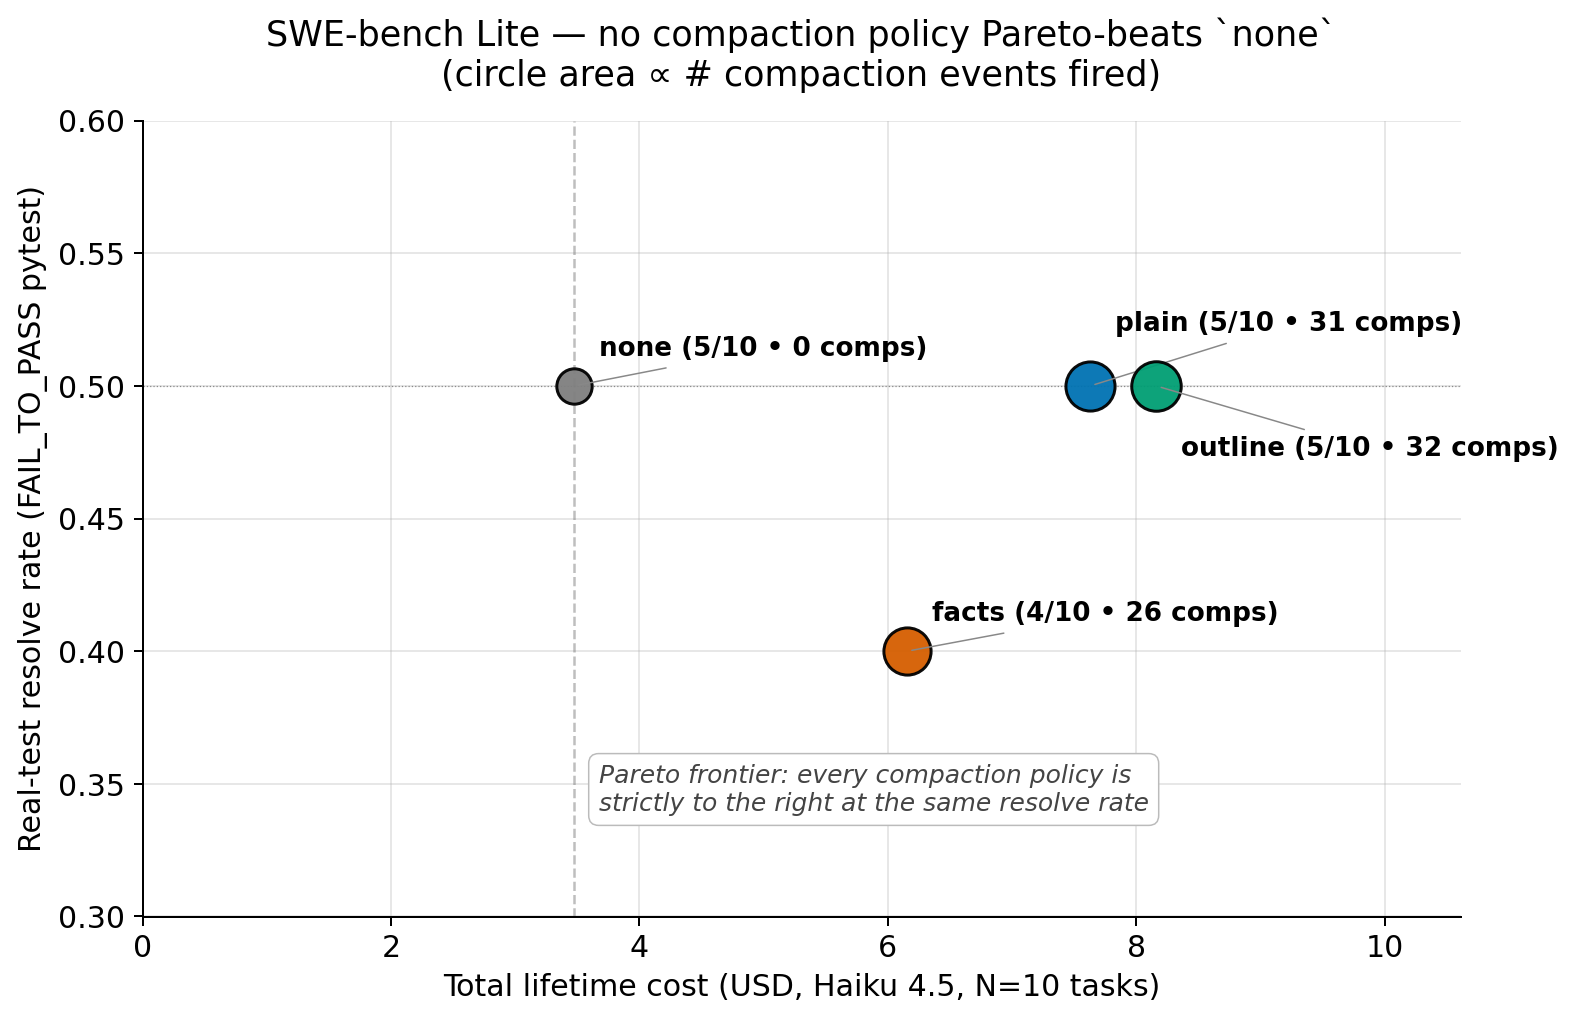
\includegraphics[width=\columnwidth]{fig1_pareto_swebench.png}
  \caption{Pareto frontier (lower-left = better). \texttt{none} is
  alone on the frontier; every compaction variant is dominated.}
  \label{fig:pareto}
\end{figure}

\begin{figure}[h]
  \centering
  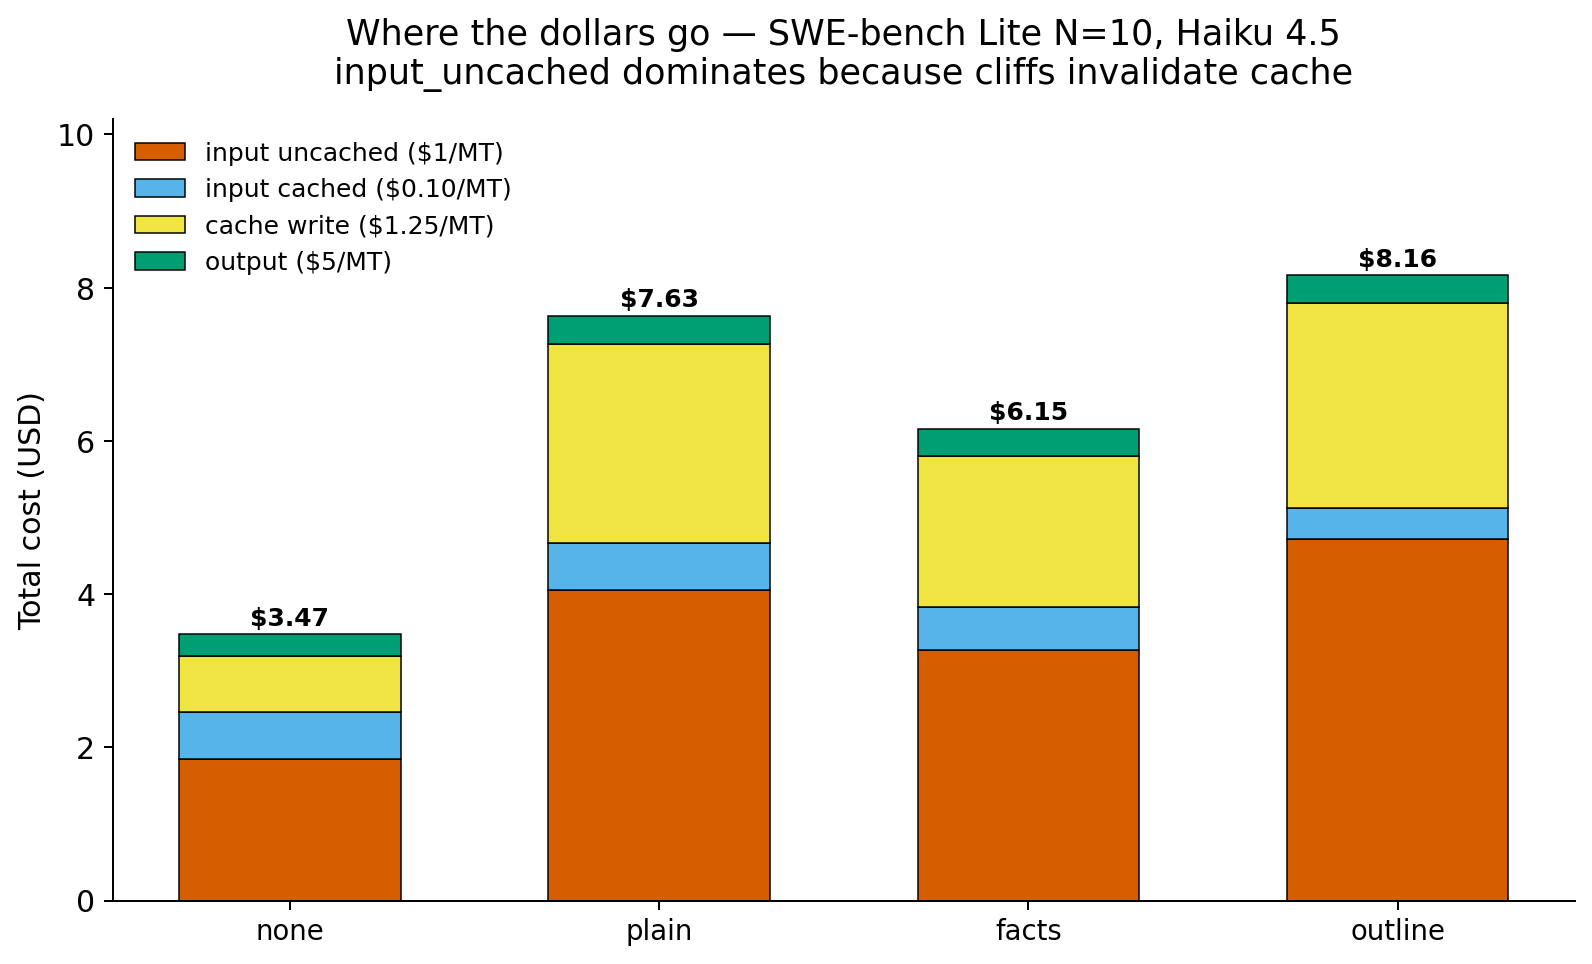
\includegraphics[width=\columnwidth]{fig2_cost_decomposition.png}
  \caption{Cost decomposition.
  \texttt{input\_uncached} dominates total cost on every compaction
  policy.  The bytes saved on dropped spans show up as reduced
  future \emph{cached} cost, which is already cheap.}
  \label{fig:cost_decomp}
\end{figure}

\begin{table}[h]
\centering\small
\setlength{\tabcolsep}{3pt}
\begin{tabular}{lcccc}
\toprule
\textbf{Policy} & \textbf{u\$} & \textbf{c\$} & \textbf{w\$} & \textbf{tot\$} \\
\midrule
\texttt{none}                & \textbf{1.155} & 0.334 & 0.000 & \textbf{1.611} \\
\texttt{llm\_reorganizer}    & 1.646 & 0.293 & 0.163 & 2.244 \\
\texttt{smart\_evict}        & 1.954 & 0.468 & 0.088 & 2.686 \\
\texttt{prefix\_preserving}  & \textbf{3.685} & 0.329 & 0.071 & \textbf{4.842} \\
\bottomrule
\end{tabular}
\caption{Cost decomposition (4 heavy SWE-bench Lite tasks).
\texttt{u\$}=input\_uncached, \texttt{c\$}=input\_cached,
\texttt{w\$}=cache\_write. \texttt{prefix\_preserving}'s 19 cliffs
generate \$3.69 of new uncached input vs \texttt{none}'s \$1.16.}
\label{tab:cost_decomp}
\end{table}


\subsection{Placeholder text affects agent behavior}
\label{sec:placeholder}

When the action-graph supersession policy compacts an
observation it leaves a short text token sequence in the prompt
where the observation used to be---the \emph{placeholder}. The
placeholder's content is a free design parameter: the eviction
signal (which observation to drop, when) is unchanged across
variants. We compared three placeholder contents: \emph{plain}
(an evicted marker only, e.g.\ \texttt{[evicted: \string~5K
tokens, consumed by edit\_file('skipping.py')]}); \emph{facts}
(the same marker plus a one-line list of the dropped file's
function names); and \emph{outline} (the same marker plus
line-numbered section headers and a ``re-read to act'' hint).

On the one validatable task where the four policies diverge, the
\emph{facts} variant performs worst: the agent fixates on the
function names exposed by the placeholder and edit-reverts on the
wrong function (18 edits, 0/2 \texttt{FAIL\_TO\_PASS}). The
\emph{plain} variant has no useful info to act on, forces a
re-fetch, and resolves in 4 edits; the \emph{outline} variant
resolves in 3. The pattern is qualitatively consistent across two
seeds, but it rests on a single task and we do not separate it
from seed variance. The observation is that placeholder
\emph{content}---a knob orthogonal to the eviction signal---can
change agent behavior; what to put in a placeholder is therefore
part of compaction-policy design, not just bookkeeping.

\subsection{Portability: rules are domain-specific}

We extended $\tau$-bench retail with a multi-customer chain
harness. At \texttt{chain\_size=10} retail, action-graph
supersession reached a max prompt of 36K (above the 29.75K trigger)
but fired \emph{zero} compactions, because retail tools
(\texttt{find\_user\_id\_by\_name\_zip}, \texttt{get\_order\_details})
do not match any of the SWE-bench-tuned supersession rules. The
signal is correct; the rule set is domain-specific. The
constructive direction is \emph{boundary-aware} supersession: any
subtask-end event consumes that subtask's tool observations.

% =====================================================================
\section{Why no policy beats \texttt{none}: the cliff tax}
\label{sec:cliff_tax}

The negative result of \S\ref{sec:results} has a single
quantitative explanation.

\subsection{Pricing}

Every modern provider bills input tokens at two rates. On Anthropic
Haiku 4.5: cached input at $\sim$\$0.10/MTok, uncached at
$\sim$\$1.00/MTok---a 10$\times$ ratio. \emph{Provider-invariant}:
holds across Sonnet, OpenAI gpt-4.1, gpt-4.1-mini, and Qwen
self-host columns.

\subsection{What a compaction event does}

The serving system keys cached blocks by chained hashes
$H_i = \mathrm{hash}(H_{i-1}, \mathrm{tokens}_i)$. Replacing a
5K-token observation at byte position 5{,}000 with a 50-token
placeholder changes $H_i$ at that position---and therefore every
$H_j$ for $j > i$. On the next request, the cache walk stops at
position 5{,}000; everything after is recomputed and re-billed at
the uncached rate. Figure~\ref{fig:chain_hash_problem} visualizes
the mechanism, and the fix our system applies.

\begin{figure}[h]
  \centering
  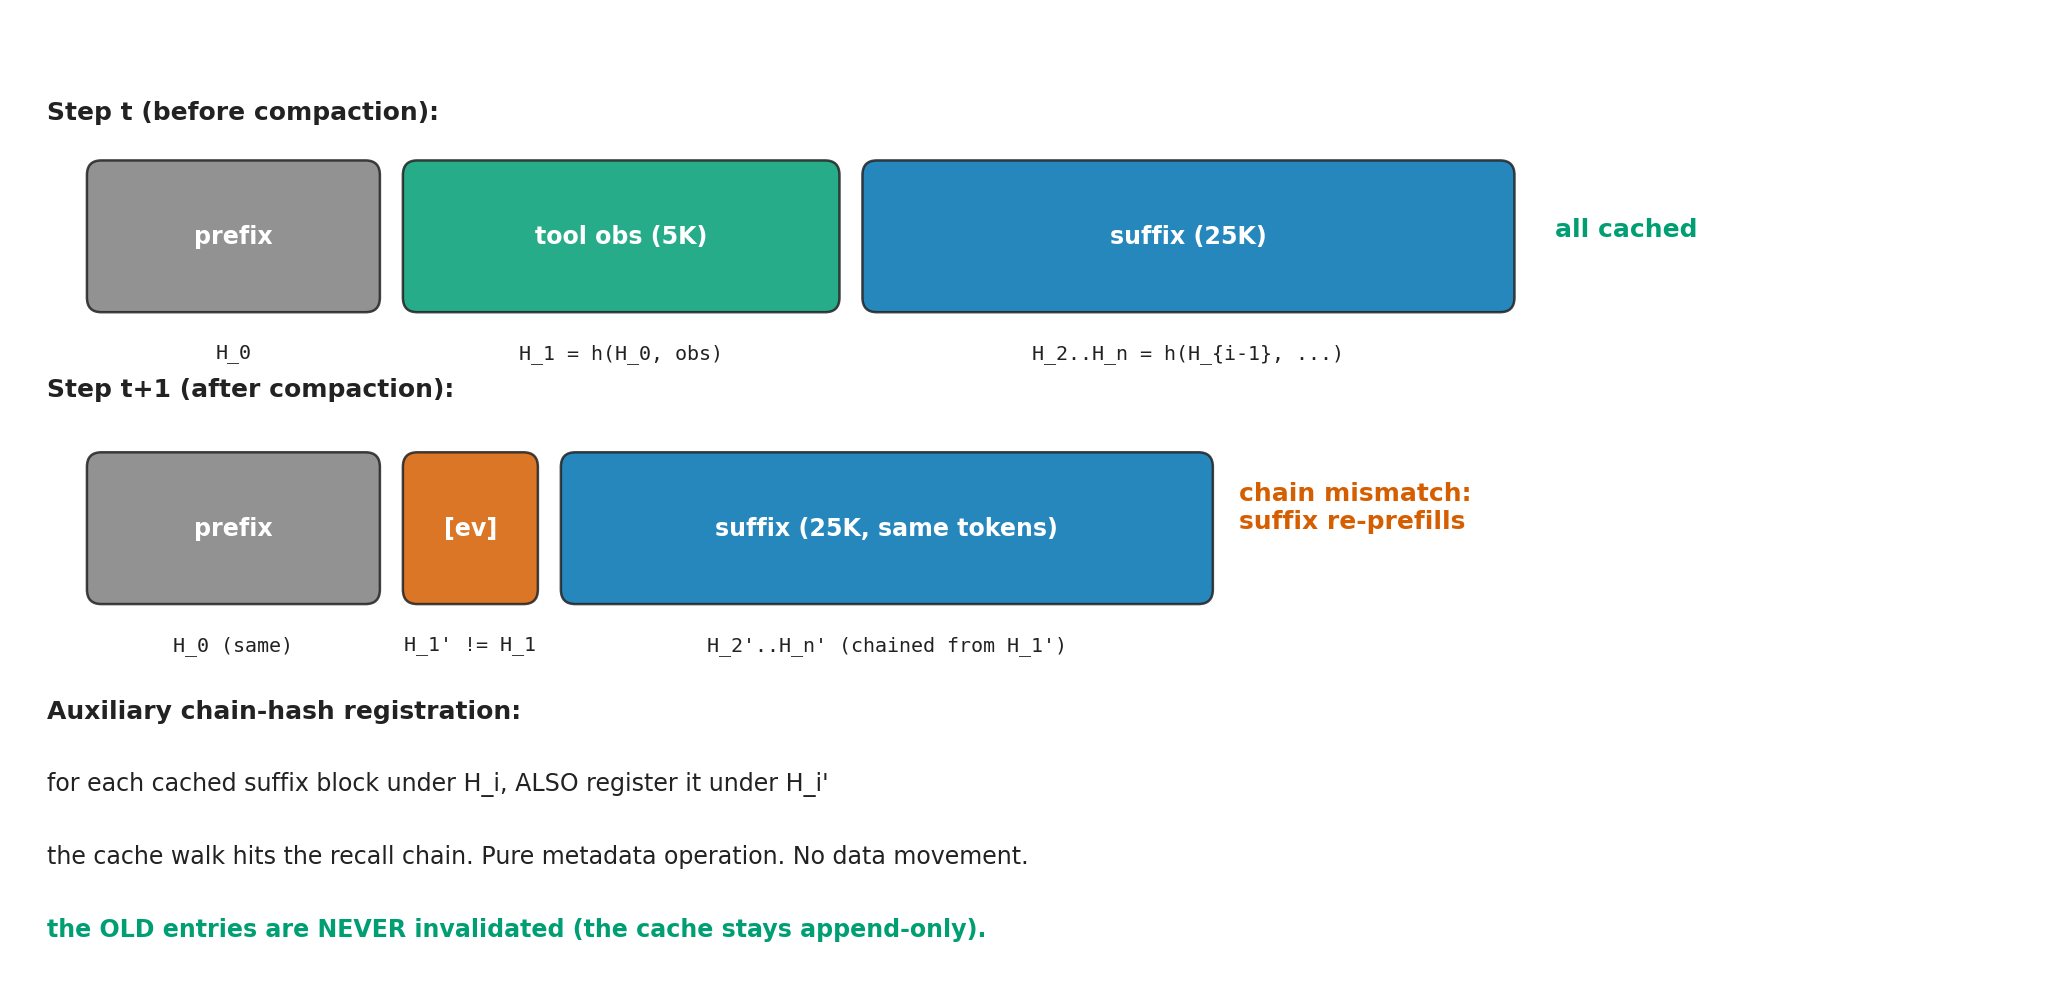
\includegraphics[width=\columnwidth]{fig_chain_hash.png}
  \caption{The chain-hash invalidation problem. The placeholder
  changes $H_1 \to H_1'$, which changes every downstream $H_j'$.
  Same suffix tokens, different cache key. Auxiliary chain-hash
  registration (bottom) restores the cache hit by adding a second
  key for the same physical blocks, append-only.}
  \label{fig:chain_hash_problem}
\end{figure}

\subsection{Break-even arithmetic}

Let $B_{\mathrm{save}}$ be bytes saved per future step,
$B_{\mathrm{rebill}}$ be bytes from the compaction position to the
prompt tail at compaction time, $r = p_u / p_c \approx 10$, and
$N$ be remaining steps after the compaction event.

Compaction saves $N \cdot B_{\mathrm{save}} \cdot p_c$ over the
remaining trajectory. It costs
$B_{\mathrm{rebill}} \cdot p_c (r-1)$ on the next call. Break-even:
\[
N \geq (r-1) \cdot \frac{B_{\mathrm{rebill}}}{B_{\mathrm{save}}}
  = 9 \cdot \frac{B_{\mathrm{rebill}}}{B_{\mathrm{save}}}
\]
Table~\ref{tab:cliff_amp} works this through with concrete
numbers under Anthropic Haiku 4.5 pricing. For a typical
compaction event
($B_{\mathrm{save}} \approx 5{,}000$,
$B_{\mathrm{rebill}} \approx 25{,}000$ at mid-trajectory),
\textbf{compaction needs $\geq 45$ remaining steps to break even}.
The trajectories in our $N{=}10$ run average $\sim$26 steps total.

\begin{table}[h]
\centering\small
\setlength{\tabcolsep}{4pt}
\begin{tabular}{lr}
\toprule
\textbf{Quantity} & \textbf{Value} \\
\midrule
Prompt size at compaction         & 30{,}000 tokens \\
Tool observation being compacted  & 5{,}000 tokens \\
Placeholder size                  & $\sim$50 tokens \\
Suffix re-billed (uncached, next call) & 25{,}000 tokens \\
\midrule
Next-call cost, cached            & \$0.0025 \\
Next-call cost, uncached          & \$0.0250 \\
$\Delta$ on next call             & \textbf{\$0.0225} \\
\midrule
Per-step savings (5K cached @ \$0.10/MTok) & \$0.0005 / step \\
Break-even ($\Delta$ / savings)   & \textbf{45 steps} \\
\bottomrule
\end{tabular}
\caption{Worked example for the break-even arithmetic at
Anthropic Haiku 4.5 pricing. A mid-trajectory compaction event
needs $\sim$45 future steps to recoup its cliff cost; agent
trajectories at the scale we tested average $\sim$26 steps.}
\label{tab:cliff_amp}
\end{table}
Compaction events usually happen mid- to late-trajectory, leaving
5--15 amortization steps. \textbf{The cliff is structurally
unrecoverable on most realistic agent trajectories.} Compaction
\emph{as a cost lever} does not beat \texttt{none}; compaction
\emph{as a behavior-modification lever} sometimes does (clearing
working memory at the right moment can change the agent's next
action), but that is not a cost story and is not what the
compaction literature claims.

% =====================================================================
\section{A cliff-free compaction substrate}
\label{sec:keep_bytes}

Re-derive the break-even with $r = 1$ (no cliff penalty):
$N \geq 0$, trivially satisfied. \emph{Any} compaction is
profitable from the first future step. The goal is therefore
simple: \textbf{when the agent compacts an observation, the
engine should keep the suffix's KV state usable; when the agent
later needs the observation back, putting it back should not
require any model recomputation.}

\para{Foundations} Our system builds heavily on the Memento
overlay~\cite{kontonis2026memento}, which introduced the idea of
representing compacted observations as inline marker tokens that
the inference engine can interpret as KV-block boundaries
without retraining the model or modifying its tokenizer.
Memento's mechanism handles the compaction direction; we extend
it with bidirectional recall---KV capture and restore, plus the
two suffix repairs described below---so that a recalled
observation costs essentially nothing beyond a memory copy.

Figure~\ref{fig:lifecycle} shows what this looks like for a
single observation across three moments in time. At $t_0$
everything is normal: the observation is in the prompt, its KV
state lives in the engine's paged cache. At $t_1$ the policy
compacts: the prompt now carries a small placeholder, and the
engine has copied the observation's KV to a CPU side cache; the
GPU blocks return to the engine's LRU pool. At $t_2$ the policy
recalls: the engine copies the saved KV back to fresh GPU blocks
at the observation's original logical position. No
recomputation; only memory movement.

The hard part is making the \emph{suffix}---the part of the
prompt written \emph{during} the compacted period---still work
after this splice. Two things go wrong with a naive splice.
First, the suffix's K vectors carry positional encoding for the
positions they had during the compacted period, not the
positions they now occupy after the observation has been
restored. Second, the prefix-cache hash table indexes those
blocks under a chain hash that runs through the placeholder, so
the recall prompt's cache walk misses. We fix the first by
rotating the cached K vectors in place by $\Delta$ tokens (a
per-layer tensor op that reuses the engine's rotary kernel and
adds no model forward pass). We fix the second by adding a
second key for the same physical blocks to the prefix-cache hash
table---append-only, never invalidating the original.

Figure~\ref{fig:architecture} shows where these operations live
in the system. The agent loop and compaction policy run in the
main process; the scheduler and GPU worker run in the
inference-engine subprocess. Four cross-process JSONL queues
(KV capture, KV restore, K rotation, auxiliary chain-hash
insert) carry the policy's decisions over the IPC boundary; the
engine drains them on each scheduling tick.

\begin{figure*}[t]
  \centering
  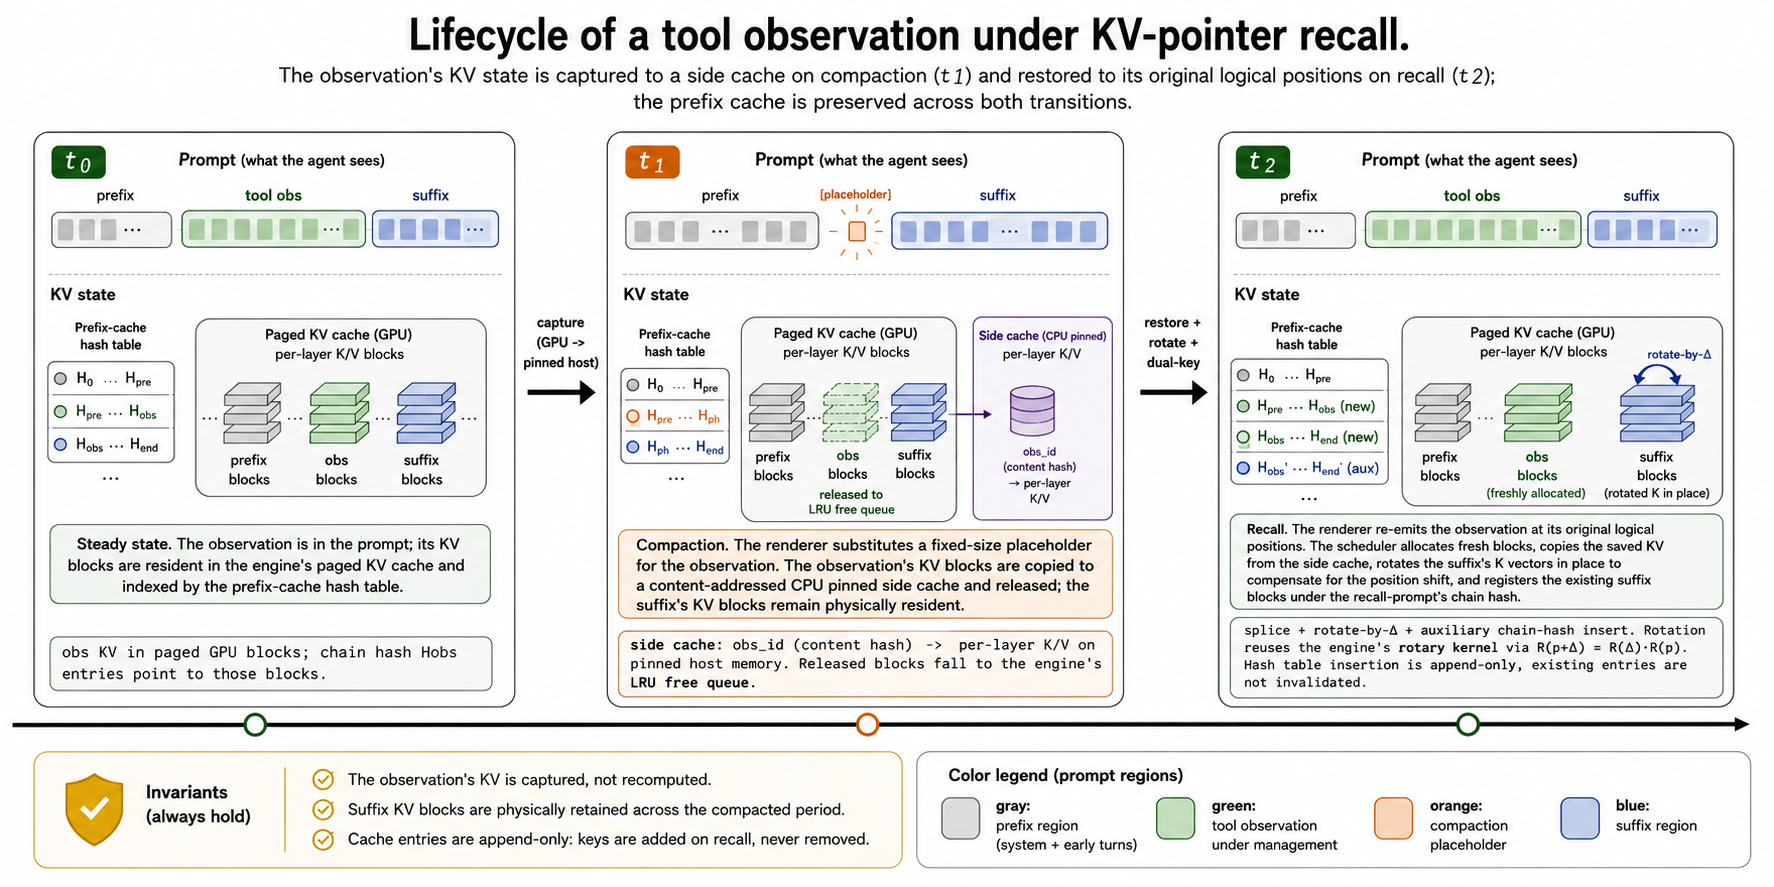
\includegraphics[width=0.97\textwidth]{lifecycle.png}
  \caption{Lifecycle of a tool observation under KV-pointer
  recall. \textbf{$t_0$} (steady state): the observation is in the
  prompt and its per-layer K/V blocks are resident in the engine's
  paged KV cache, indexed by the prefix-cache hash table.
  \textbf{$t_1$} (compaction): the renderer substitutes a
  fixed-size placeholder for the observation; the engine captures
  the observation's K/V to a content-addressed CPU pinned side
  cache and releases the GPU blocks; the suffix's blocks remain
  physically resident but become reachable only under a
  compacted-period chain hash. \textbf{$t_2$} (recall): the engine
  allocates fresh blocks, restores the saved K/V from the side
  cache, rotates the suffix's K vectors in place by $\Delta$
  tokens to compensate for the position shift, and registers the
  existing suffix blocks under the recall-prompt's chain hash.
  Three invariants hold across the lifecycle: the observation's K/V
  is captured (not recomputed), the suffix blocks are physically
  retained, and prefix-cache entries are append-only.}
  \label{fig:lifecycle}
\end{figure*}

\begin{figure*}[t]
  \centering
  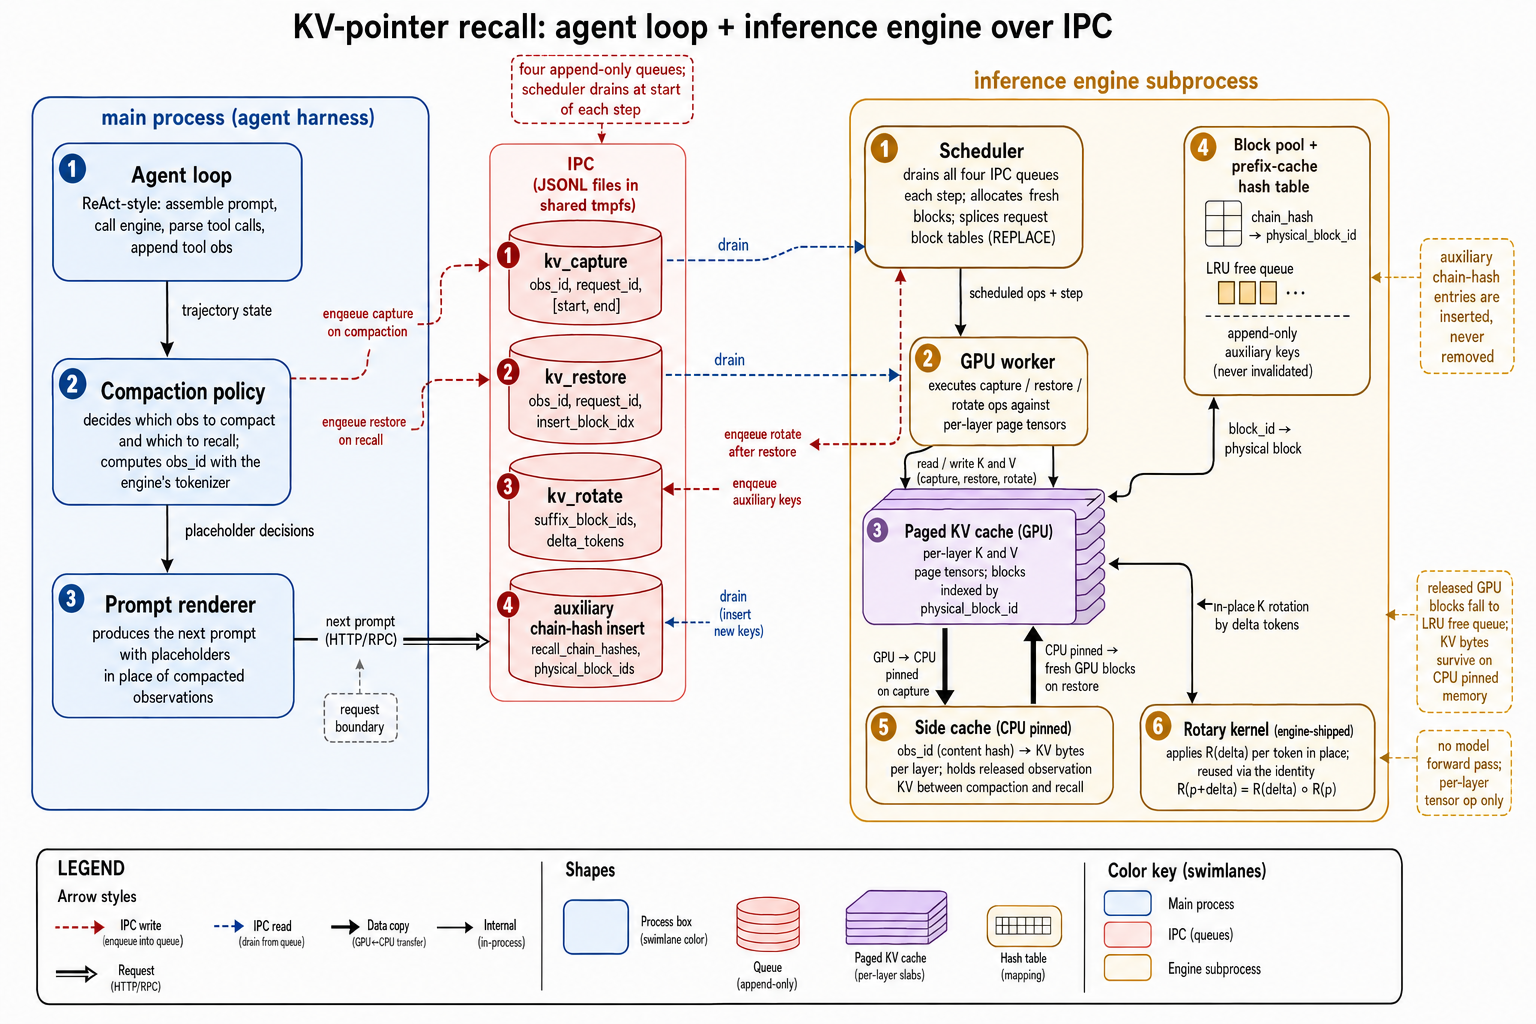
\includegraphics[width=0.97\textwidth]{architecture.png}
  \caption{System architecture. The agent loop, the compaction
  policy, and the prompt renderer run in the main process; the
  scheduler and GPU worker run in the inference-engine subprocess.
  Coordination across the boundary is via four append-only
  JSON-line queues in shared tmpfs (KV capture, KV restore, K
  rotation, auxiliary chain-hash insert) drained by the scheduler
  on each step. A content-addressed side cache lives engine-side
  and holds CPU pinned K/V for released observations; the rotary
  kernel and prefix-cache hash table are reused unmodified from
  the engine. Hash determinism across the process boundary
  requires matching tokenizer and PRNG seed; hashing the wrong
  tokenizer was an early build bug.}
  \label{fig:architecture}
\end{figure*}

\subsection{Why text-level recall isn't enough}

The naive recall is text-level: substitute the original observation
for its placeholder in the prompt and let the engine re-prefill.
Two variants---in-place (at the original position) and append
(at the prompt tail)---differ in how much of the suffix the
re-prefill catches. Figure~\ref{fig:cache_hit_recall} reports
cache hit rates from an evaluation in which the engine's normal
LRU eviction is allowed to release blocks (rather than
refcount-pinning the observation's blocks): in-place recall eats
a 27-point cache penalty relative to a no-recall control,
even though the suffix tokens themselves are unchanged. The
penalty is purely a chain-hash mismatch: the suffix's parent
chain runs through the original observation in the recall prompt
but through the placeholder in the cache. The fix is engineering
the cache to hold both keys.

\begin{figure}[h]
  \centering
  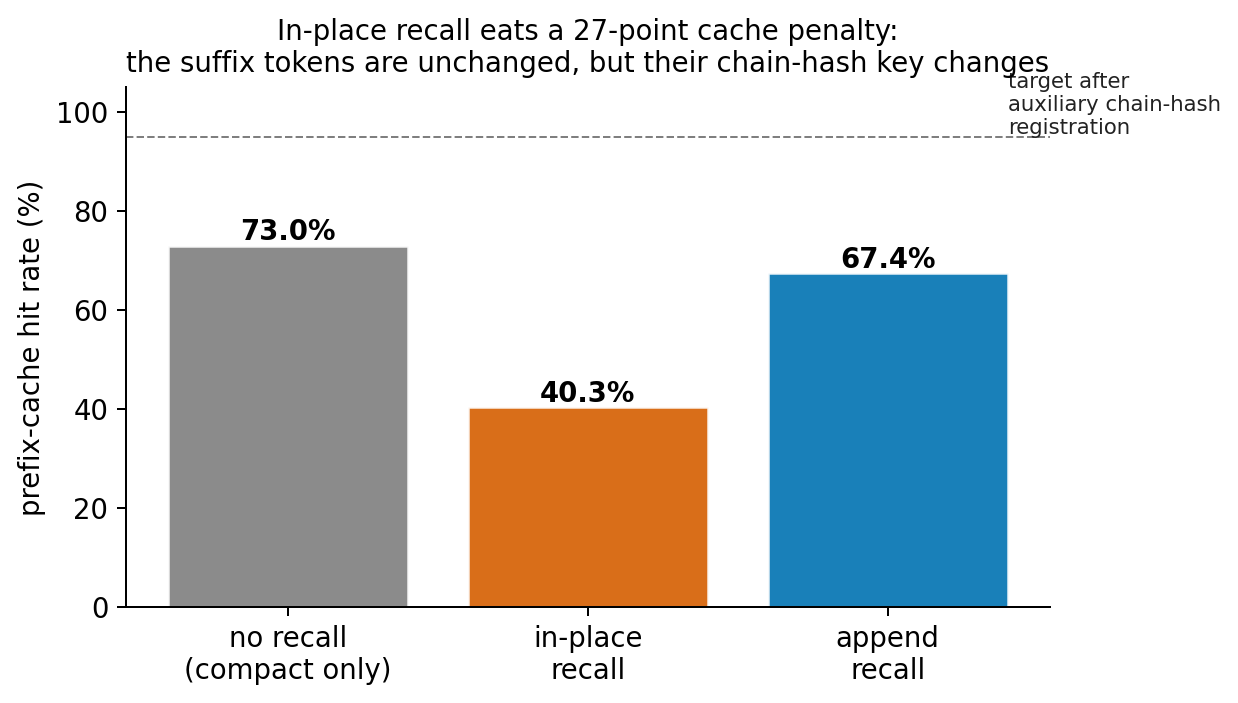
\includegraphics[width=\columnwidth]{fig_cache_hit_recall.png}
  \caption{Cache hit rate across text-level recall variants.
  In-place recall loses 27 points to no-recall despite identical
  suffix tokens; the penalty is the chain-hash mismatch.}
  \label{fig:cache_hit_recall}
\end{figure}

\subsection{KV-level mechanisms in the engine}

The full mechanism (Figure~\ref{fig:lifecycle}, $t_1 \to t_2$)
combines three engine-side operations on top of a side cache.

\para{Side cache: capture and restore} At $t_1$, the engine copies
the observation's K/V from GPU to CPU pinned memory and indexes
it by a content hash; the GPU blocks are released without a
refcount pin and fall to the engine's LRU free queue. At $t_2$,
the scheduler allocates fresh GPU blocks via the engine's
allocator, queues a CPU$\to$GPU memcpy, and splices the new
blocks into the request's block table at the original logical
position. The splice must \emph{replace} the affected slice of
the block-table list; an insert grows the table and overshoots
\texttt{num\_computed\_tokens} on a later step, tripping a
scheduler assert.

\para{In-place rotary K rotation} Modern LLMs (Qwen3 included)
encode token position via rotary positional
embedding~\cite{su2024rope} (RoPE): each token's K vector is
rotated by an angle proportional to its absolute position, with
the rotation applied at compute time and ``baked'' into the
stored K. After the splice above, the suffix's K vectors carry
the angles they had during the compacted period, but their
logical positions have shifted by
$\Delta = m_{\mathrm{obs}} - p_{\mathrm{placeholder}}$ tokens
(the obs's $\sim$5K tokens replace the placeholder's $\sim$50).
For $\Delta \approx 5000$, high-frequency rotary channels wrap
many times around the unit circle and suffix attention becomes
random.

Rotary embeddings compose: $R(p+\Delta) = R(\Delta) \circ R(p)$.
Multiplying the cached suffix K vectors by $R(\Delta)$ in place
corrects their phase without any model forward pass. The
operation is per-layer, fixed-shape, and reuses the engine's
shipped rotary kernel. We verified composition with three
microbenchmarks: in fp32, cosine similarity \textbf{1.0000000}
across all $(p, \Delta)$ pairs tested; the engine kernel
composes the same way; in bf16 in the paged KV layout, cosine
similarity exceeds 0.999 across layers and V tensors are
bit-identical pre/post.

\para{Auxiliary chain-hash registration} For each cached suffix
block under the compacted-period chain hash, the scheduler
\emph{also} inserts it into the prefix-cache's hash table under
the recall-prompt's chain hash. Pure metadata operation---no data
movement, no kernel work, append-only. The \emph{old} entries
are never invalidated, a project-wide invariant: future requests
that walk the old chain still find the same physical blocks. The
storage-systems insight is that the engine's prefix cache is
content-addressable and position-immutable by default; we make it
position-mobile by \textbf{adding} new keys, not removing old
ones.

\para{End-to-end test} On a single SWE-bench Lite task
(Qwen3-30B, H100), the engine stats record three captures, four
restores, and two rotations covering 1260 blocks. The salient
number is \textbf{zero refcount pins applied}: the captured GPU
blocks were not pinned, the request truncation released them
under LRU pressure, and the recall still recovered correct KV
state. Block-level release is directly observed in a parallel
memory trace---the scheduler's free-block count oscillates across
capture / restore / rotate events as expected.

\para{Engine-side capacity returned} A complementary measurement:
under \texttt{--no-pin}, captured observation blocks fall to the
engine's LRU free queue and become reusable by other concurrent
requests on the same engine. On a 14-step \texttt{lru-kvrestore}
trajectory of \texttt{pytest-7490} (Qwen3-30B-A3B, bf16, GQA with
4 KV heads, 16-token blocks at 1.50\,MB each), the GPU memory
trace records a peak instantaneous free-block delta of 988
blocks ($\approx$1.55\,GB) and a cumulative 1973 blocks
($\approx$3.10\,GB) recycled into the free pool across 12
capture events. The mechanism's own GPU work (capture / restore
/ rotate) totals 1.78\,s out of 87.3\,s of engine wall
($\approx$2\%), so this capacity return is essentially free. We
do \emph{not} claim memory release to the OS: PyTorch's caching
allocator never shrinks (\texttt{alloc\_bytes} stayed constant
at 73.2\,GB), so other Linux tenants still see the GPU as fully
occupied. The win is internal to the engine. In a multi-agent
serving topology where one engine serves $N$ concurrent agents,
every $\approx$1.5\,GB returned per agent trajectory is one
additional concurrent working set fitting in the same hardware
budget; the gain scales linearly with compaction events per
trajectory.

\subsection{Alternative: attention-mask eviction}

An alternative to moving KV bytes is to leave the observation's
blocks pinned in their GPU positions and toggle attention
\emph{off} during the compacted period via the request's
masked-block list; recall becomes a mask flip. In
mechanism-internal comparisons, mask-based eviction wins by
$-55\%$ wall on the regime with the most compaction events and
loses on light-compaction regimes where the marker tax dominates;
on a four-task four-seed recall-heavy evaluation, attention-unmask
recall beats text-append recall by $-11\%$ wall mean. The
trade-off is structural: mask-based trades GPU bytes for engine
simplicity. Neither is a comparison to \texttt{none}.

\subsection{Engineering effort}

Getting the mechanism end-to-end took three days of continuous
engineering and a sizeable patch set against vLLM. The final
delta is \textbf{+2225 / $-$44 lines across 12 files in
\texttt{vllm/v1/}} on top of a pinned base commit, landed across
33 commits. The bulk of the change is in two files: the
scheduler (\texttt{sched/scheduler.py}, 19 hunks containing most
of the capture / restore / rotate / dual-key control flow) and
the GPU worker (\texttt{worker/gpu\_model\_runner.py}, +461 lines
covering the K-rotation kernel call, the splice execution path,
and the GPU memory trace). The remainder is split between the
single-type KV-cache manager (capture / restore / rotate
plumbing), the block-masking overlay
(\texttt{core/block\_masking/} — \texttt{memento\_store},
\texttt{tracker}, package init), and smaller hunks in the block
pool, the KV-cache manager, the scheduler-output struct, the
request struct, and configuration plumbing. Two patches were
reverted in-session because they would have violated the
project-wide ``never invalidate'' invariant
(\S\ref{sec:keep_bytes}).

The recurring source of difficulty is structural rather than
algorithmic: the system has \emph{four} cross-process state
surfaces (Figure~\ref{fig:architecture}) and \emph{two}
tokenizers, and any divergence between policy-side and
engine-side views manifests as either a silent recall miss or a
hard scheduler assert. Representative classes of issue: vLLM API
drift between minor releases (pin to a specific commit, not a
release tag); a tokenizer mismatch on the obs-id content hash
that prevented recall from ever matching until both sides routed
through the engine's tokenizer; a block-table splice that grew
the table by inserting rather than replacing the affected slice,
eventually overshooting \texttt{num\_computed\_tokens} on a
later step; stale chain-hash entries under no-pin operation,
patched with defensive clamps because the principled fix would
have required invalidating cache entries.

% =====================================================================
\section{What we have not shown}
\label{sec:status}

We are deliberate about distinguishing \emph{mechanism progress}
from \emph{empirical Pareto-win against the baseline}. The
KV-pointer recall mechanism is end-to-end operational; the
Pareto-win against \texttt{none} on a real task list
\textbf{has not yet been measured}. The project was compute-bound
throughout; an end-to-end head-to-head run did not land within
our budget.

\para{Phase status at submission} A validation run that forces
recall on every memento'd observation
(\texttt{pytest-7490}, Qwen3-30B-A3B, two seeds, max\_steps=20,
\texttt{recall\_low\_water=2.0}, \texttt{--no-pin}) survives 12
successive captures and 12 successive recalls without crashing,
returns $\approx$1.55\,GB of GPU KV blocks to the engine's free
pool at peak, and pays $\sim$2\% of engine wall on the
splice/restore/rotate work itself. \textbf{The remaining honest
gap is a $+57\%$ per-step wall over the no-compaction baseline on
the same trajectory.} That gap is not the rotation mechanism; it
is prefill cost on tokens that should have been cache hits. We
traced it to chain-hash mutations introduced when the renderer
transitions between mementoed and un-mementoed forms of a
message. One transition (the first time an observation is
mementoed) is now closed by a renderer change that always emits
\texttt{<tool\_response>...</tool\_response>} markers, so with-
and without-memento renderings differ only in their appendix
bytes. The other (un-mementoing on recall) remains open: the
auxiliary chain-hash registration of \S\ref{sec:keep_bytes} is
the intended fix, the engine-side code is wired, but in our most
recent run the trigger did not fire in production
(\texttt{dual\_key\_inserts}=0). The fix in flight is to invoke
the auxiliary insert on every recall regardless of rotation
delta; this is not validated in this report.

\begin{itemize}[itemsep=2pt,topsep=2pt]
\item \textbf{No apples-to-apples mechanism vs.~\texttt{none}.}
Single-task end-to-end tests do not overlap with the small task
list where we measured the \texttt{none} baseline. Vanilla
baseline = 1/5 resolved on that list; a future list with a higher
resolve ceiling is preferable.
\item \textbf{Recurring scheduler assert.}
\texttt{total\_num\_scheduled\_tokens$>$0} occasionally trips on
long evaluations. Patched with defensive clamps; not fixed at root.
The likely cause is the stale chain-hash entries described above.
\item \textbf{Multi-seed at $N{=}10$ for the main result.} The
single-seed run gives the negative result; a multi-seed run is
needed to bound the seed-driven per-task variance flagged in
\S\ref{sec:placeholder} and confirm the Pareto outcome.
\end{itemize}

\section{Future work}
\label{sec:future}

The most direct next steps, all gated on compute rather than
design:

\begin{itemize}[itemsep=2pt,topsep=2pt]
\item \textbf{Apples-to-apples mechanism vs.~\texttt{none}.}
A shared task list with multi-seed evaluation under both
configurations. This is the missing empirical comparison the
constructive direction needs.
\item \textbf{Multi-seed N=10 main result.} 3 seeds × 4 policies
× 10 tasks. Replaces the single-seed numbers with a paired test.
\item \textbf{End-to-end validation of the auxiliary chain-hash
registration} on a recall-heavy workload, looking for the
predicted 40\% $\to$ $>$90\% in-place-recall cache-hit jump.
\item \textbf{Boundary-aware supersession.} Add a rule that any
subtask-end event consumes that subtask's tool observations and
re-run the multi-customer chain evaluation, where the
SWE-bench-tuned rules currently fire zero compactions.
\item \textbf{Long-context regimes.} The cliff-tax derivation
predicts compaction's penalty shrinks once trajectories are long
enough to amortize the re-prefill; the inflection point is an
empirical question we did not reach.
\item \textbf{A Yellow-Pages-style benchmark.} SWE-bench Lite
trajectories are largely linear---the agent reads, edits, and
moves on, with limited revisits to earlier observations. A
benchmark in which the agent must repeatedly look up
information across many entries (think directory-style
lookups, where an observation seen at step $k$ is needed again
at step $k{+}40$) would exercise compaction \emph{and} recall
together at high frequency. This is exactly the regime where
KV-pointer recall amortizes its overhead: each compaction-recall
cycle reuses the cached suffix instead of re-prefilling it. We
expect the cliff-free substrate to show its strengths here in a
way SWE-bench Lite cannot.
\end{itemize}

The closest thing we have to a positive number for the
constructive direction is the recall-heavy mechanism-internal
comparison ($-11\%$ wall, mask vs append recall), which is a
within-mechanism comparison and not a comparison to
\texttt{none}.

% =====================================================================
\section{Goal achievement}
\label{sec:goals}

\para{75\% (baseline + simple pruning)} Achieved. \texttt{none},
FIFO, and position-aware placeholder eviction implemented and
measured across SWE-bench Lite live and $\tau$-bench retail with
real Anthropic cache-read accounting.

\para{100\% (\sysname{} compaction + reordering, full comparison)}
Eight training-free policies implemented and compared
(\S\ref{sec:policies}); the comparison shows none beats
\texttt{none} at the scale tested. Reordering as a static-prompt
operation was \emph{not} pursued: the cliff-tax analysis
(\S\ref{sec:cliff_tax}) showed it could not pay off without
changing the cost model itself.

\para{Pivot} On finding that the cliff is structural, we redirected
effort from heuristic scorers (the original 125\% goal: an MLP
scorer trained on attention oracle labels) to attacking the cliff
directly. The result is the engine overlay of
\S\ref{sec:keep_bytes}: KV capture/restore, in-place rotary
rotation, and append-only auxiliary chain-hash registration. This
is a different program from the original 125\% but it subsumes the
layout-reorganization goal: the auxiliary chain-hash registration
is the storage-systems primitive that makes ``re-position cached
blocks without paying for it'' actually possible.

% =====================================================================
\section{Conclusion}
\label{sec:conclusion}

We set out to test whether layout-aware, training-free heuristic
compaction can Pareto-dominate no compaction on the lifetime cost
of LLM agents. Across the policies, models, and benchmarks
tested, the answer is no. The reason is the cliff tax:
byte-level eviction structurally costs more on the next call
than it saves over the remaining trajectory, on the agent
workloads at the scale we evaluated.

Inside the negative result we report two findings worth keeping:
an action-graph supersession signal that uses agent tool-call
semantics to identify provably stale tool observations, and an
observation that placeholder content is its own design knob, with
two placeholder texts under the same eviction signal producing
qualitatively different agent trajectories.

The constructive direction is to change the cost model
itself---to make the cached suffix remain reachable and correct
even after the prompt prefix changes. We built an inference-engine
overlay that does this through KV capture and restore, in-place
rotary rotation of the suffix's K vectors, and append-only
auxiliary chain-hash registration. The mechanism is verified
end-to-end on H100; the empirical demonstration that the
resulting recall is genuinely cheaper than \texttt{none} is the
missing comparison.

The takeaway: prefix-cache reuse is determined by chain-hash
invariants, not by which bytes look stale. Any compaction policy
that mutates the prompt prefix without preserving the cached
suffix's reachability under the new chain hash pays the cliff
tax this report measures.

% =====================================================================
\bibliographystyle{plain}
\bibliography{refs}

\end{document}
